% This file is meant to be included in another 
\documentclass{article}
\usepackage{epsfig}

\begin{document}
\section{{\tt Dirichlet()}}

\subsection{Purpose}

Calculates the values of the Dirichlet kernel ${\cal D}_N(x)$ for 
discrete values of $x$ starting at $x=0$..

\subsection{Synopsis}

% Syntax: argument definitions, calling signature

\begin{verbatim}
#include "Dirichlet.h"

void 
Dirichlet( Status*, REAL4Vector*, DirichletParameters* )

typedef struct tagDirichletParameters{
  INT4   n;       /* Dirichlet parameter N */
  INT4   length;  /* specified length of output vector */
  REAL8  deltaX;  /* spacing of x values */
} DirichletParameters; 
\end{verbatim}

\subsection{Description}

{\tt Dirichlet()} calculates the values of the Dirichlet kernel
defined by \cite{PW}:
%
\[
{\cal D}_N(x):=
\left\{
\begin{array}{cl}
(-1)^{x(N-1)} & \quad x=0, \pm 1, \pm 2, \cdots\\
{\sin(N\pi x)\over N\sin(\pi x)} & \quad {\rm otherwise}\ .
\end{array}
\right.
\]
%
The magnitude of the Dirichlet kernel is $1/N$ times the magnitude 
of the discrete Fourier transform of the discrete $N$-point rectangular 
window.

\subsection{Operating Instructions}

% Detailed usage 

\begin{verbatim}
Status                  status; 
REAL4Vector*            poutput = NULL; 
DirichletParameters     parameters;

/* choose input parameters */
parameters.n      =  10;
parameters.length = 101;
parameters.deltaX = .01;

/* create vector */
SCreateVector( &status, poutput, parameters.length );

/* calculate values of the Dirichlet kernel */
Dirichlet ( &status, poutput,  &parameters ); 

...

/* destroy vector */
SDestroyVector( &status, &poutput );
\end{verbatim}

\subsubsection{Arguments}

% Describe meaning of each argument

\begin{itemize}
\item 
{\tt status\/} is a universal status structure. 
Its contents are initially assigned by {\tt INITSTATUS()\/} and then 
set by {\tt Dirichlet()\/} on return. 
Non-zero status codes indicate an error condition as specified in 
Table~\ref{tbl:Errors}.
\item 
{\tt poutput\/} is a pointer to a structure of type {\tt REAL4Vector}. 
One must call {\tt SCreateVector()\/} to allocate storage for the
values of the Dirichlet kernel.
The length of the output vector must equal the length specified in 
the input parameters or an error will occur.
Upon successful return from {\tt Dirichlet()\/}, {\tt poutput->data\/}
contains the values of the Dirichlet kernel ${\cal D}_N(x)$ evaluated 
at the discrete set of values 
$0, \Delta x, 2\Delta x, \cdots, (M-1)\Delta x$,
where $N={\tt parameters.n\/}$, $M={\tt parameters.length\/}$,
and $\Delta x={\tt parameters.deltaX\/}$,.
\item 
{\tt parameters\/} is a structure of type {\tt DirichletParameters\/}.  
{\tt parameters.n\/} is the Dirichlet parameter $N$;
it is an integer that must be $> 0$.
{\tt parameters.length\/} is the specified length of the output vector;
it is also an integer that must be $> 0$.
{\tt parameters.deltaX\/} is a double precision value containing the
value of $\Delta x$, which must be $>0$.

\end{itemize}

\subsubsection{Options}

None.

\subsubsection{Error conditions}

% What constitutes an error condition? What do the error codes mean?

{\tt Dirichlet()\/} sets the universal status structure on return. 
Non-zero status codes indicate an error condition. 
Error conditions are described in Table~\ref{tbl:Errors}.

\begin{table}
\begin{center}
%\hskip -0.7in
\begin{tabular}{|r|l|l|}\hline
status & status & Description\\
code   & description &\\
\hline
ENULLIP	& {\tt \&parameters == NULL\/} 
& Pointer to input parameters must be non-null\\
ENVALUE & {\tt parameters.n $\le$ 0} 
& Dirichlet parameter $N$ must be $>0$\\
ESIZE & {\tt parameters.length $\le$ 0} 
& Specified length of output vector must be $>0$\\
EDELTAX & {\tt parameters.deltaX $\le$ 0} 
& Spacing of $x$ values must be $>0$\\
ENULLOP & {\tt poutput == NULL\/}
& Pointer to ouput vector must be non-null\\
ESIZEMM & {\tt poutput->length !=\/}
& Length of output vector must agree\\
& {\tt parameters.length\/} 
& with length specified in input parameters\\
ENULLD & {\tt poutput->data == NULL\/}
& Pointer to data member of output vector must\\
&& be non-null\\
\hline
\end{tabular}
\end{center}
%
\caption{Error conditions for {\tt Dirichlet()\/}}
\label{tbl:Errors}
\end{table}
                                
\subsection{Algorithms}

% Describe algorithm by which work is done

None.

\subsection{Accuracy}

% For numerical routines address issues related to accuracy:
% approximations, argument ranges, etc.

The values of the Dirichlet kernel are calculated in single precision.

\subsection{Tests}

% Describe the tests that are part of the test suite

The program {\tt DirichletTest()} tests the function {\tt Dirchlet()}.
It tests all error conditions listed in Table~\ref{tbl:Errors}.
It also writes to files the values of the Dirichlet kernel for three
different valid test cases.
(See Figs.~\ref{f:fig1}-\ref{f:fig3}.)

\subsection{Uses}

% What LAL, other routines does this one call?

{\tt Dirichlet()\/} calls no other routines.

\subsection{Notes}

None.

\subsection{References}

% Any references for algorithms, tests, etc.

\begin{thebibliography}{0}
\bibitem{PW}
{\em Spectral analysis for physical applications},
by Donald B.\ Percival and Andrew T.\ Walden
(Cambridge University Press, Cambridge, 1993), p.\ 26-27.
\end{thebibliography}

% figures %%%%%%%%%%%%%%%%%%%%%%%%%%%%%%%%%%%%%%%%%%%%%%%%%%%

\begin{figure}[htb!]
\begin{center}
\noindent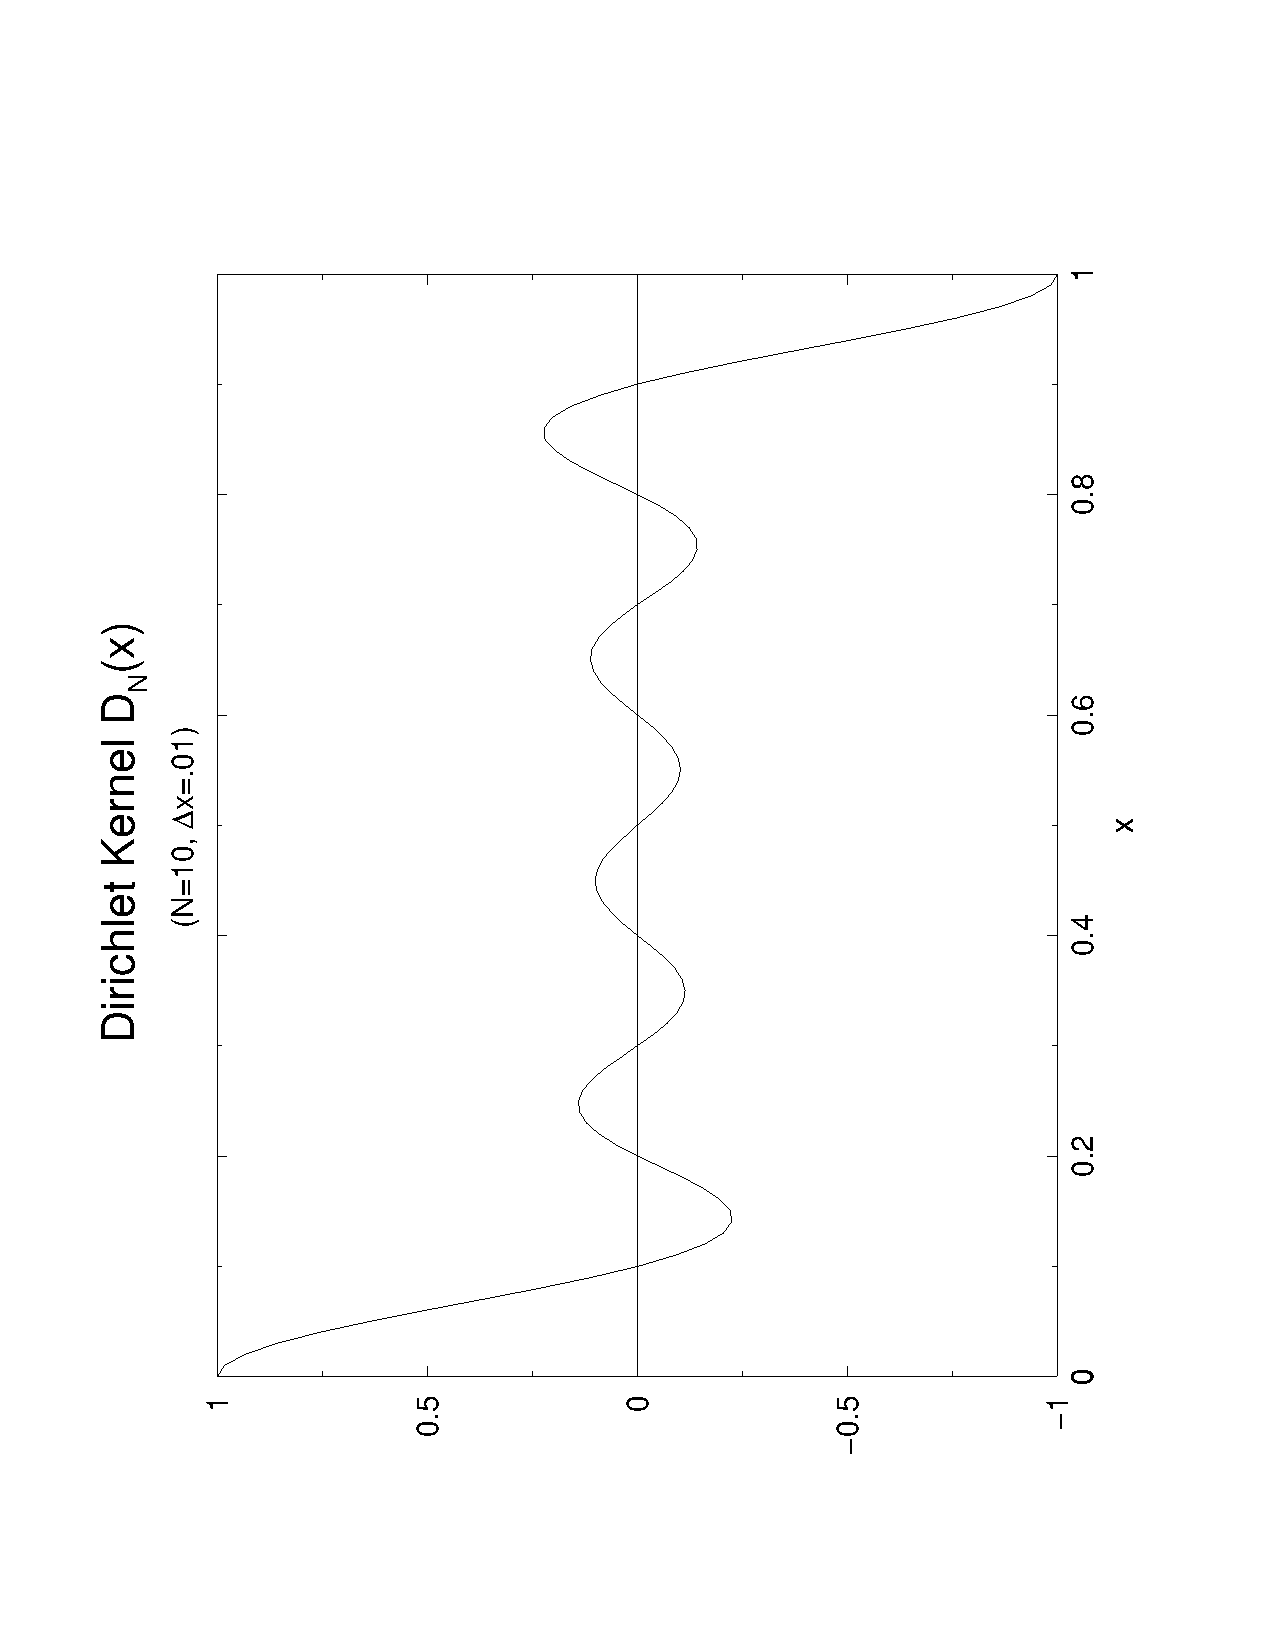
\includegraphics[angle=-90,width=4in]{fig1}
%{\psfig{file=fig1.ps,
%angle=-90,width=4in,bbllx=25pt,bblly=50pt,bburx=590pt,bbury=740pt}}
\caption{\label{f:fig1}
Dirichlet kernel for $N=10$, $\Delta x =.01$, and $0\le x\le 1$.}
\end{center}
\end{figure}
%
\begin{figure}[htb!]
\begin{center}
\noindent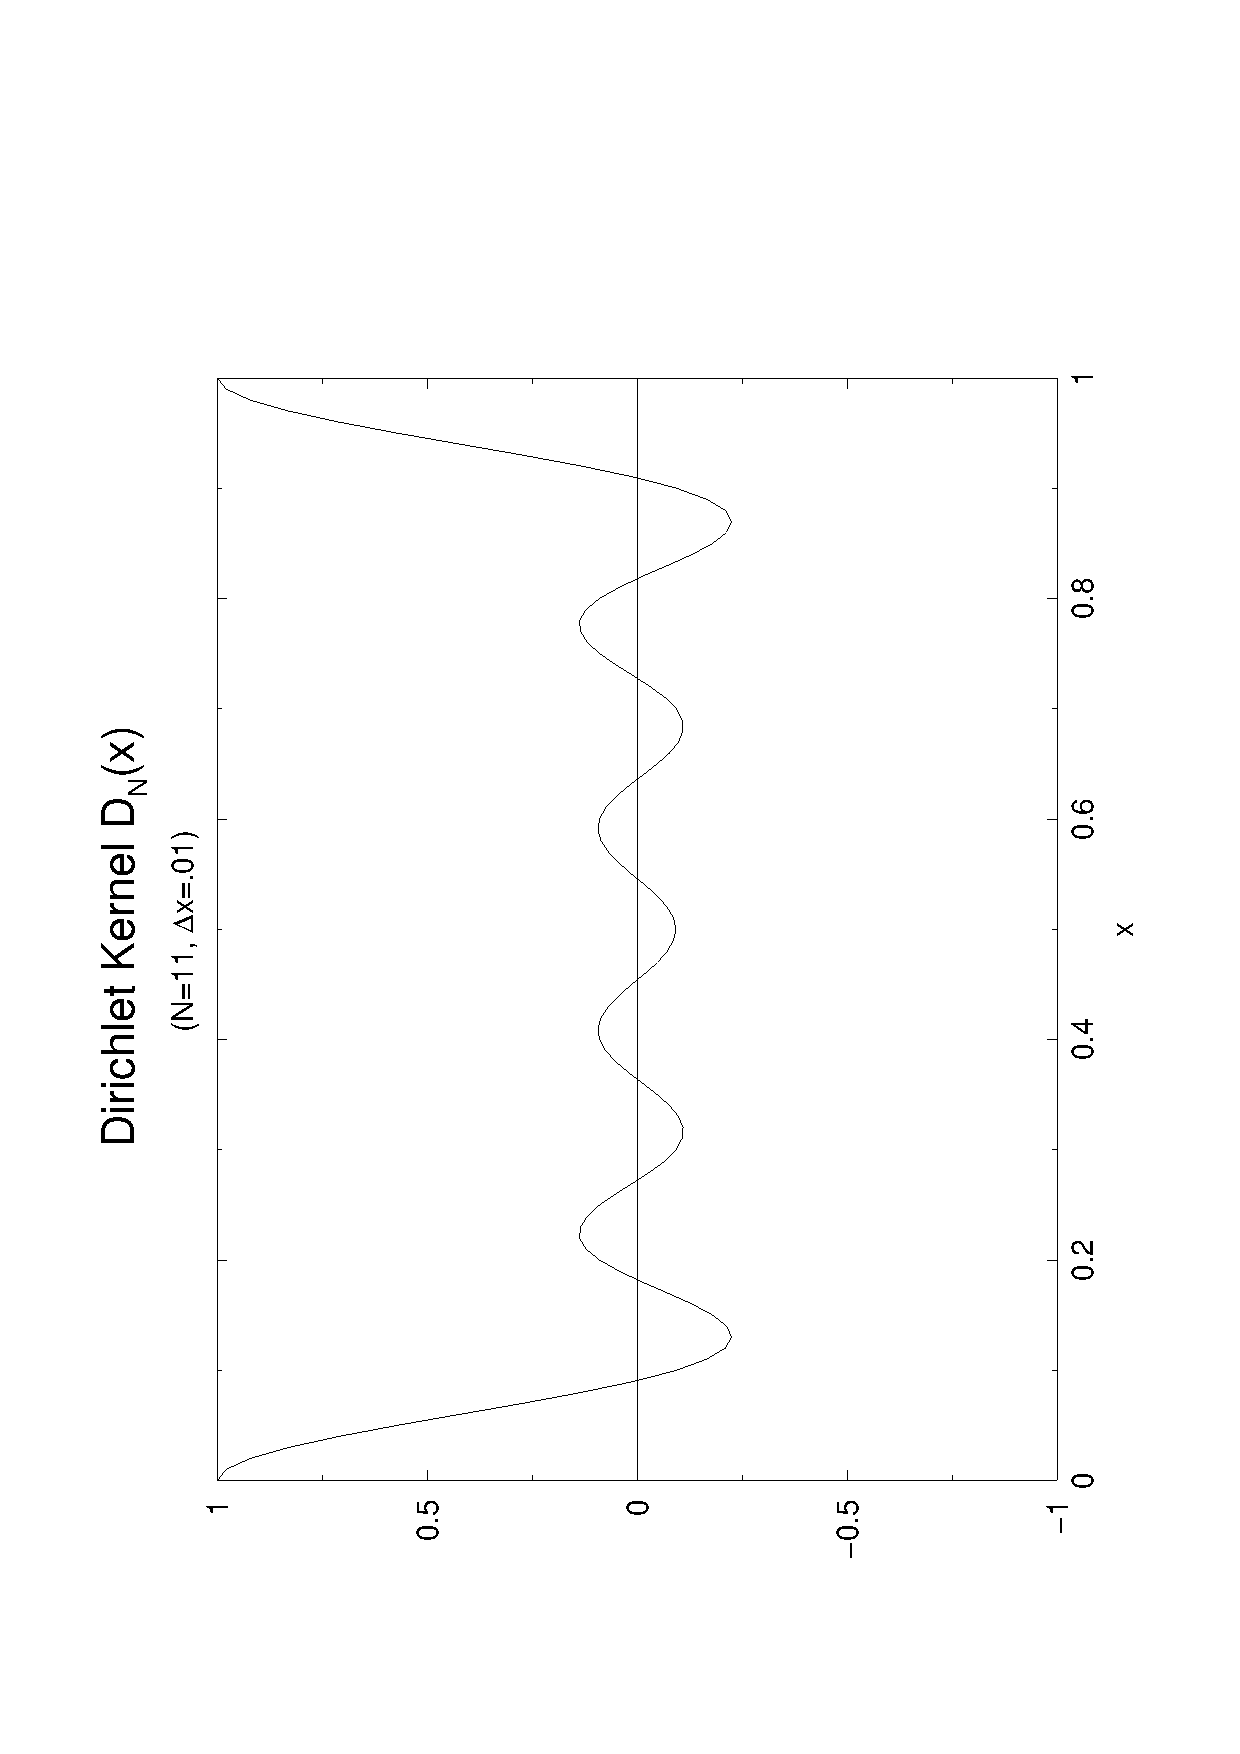
\includegraphics[angle=-90,width=4in]{fig2}
%{\psfig{file=fig2.ps,
%angle=-90,width=4in,bbllx=25pt,bblly=50pt,bburx=590pt,bbury=740pt}}
\caption{\label{f:fig2}
Dirichlet kernel for $N=11$, $\Delta x =.01$, and $0\le x\le 1$.}
\end{center}
\end{figure}
%
\begin{figure}[htb!]
\begin{center}
\noindent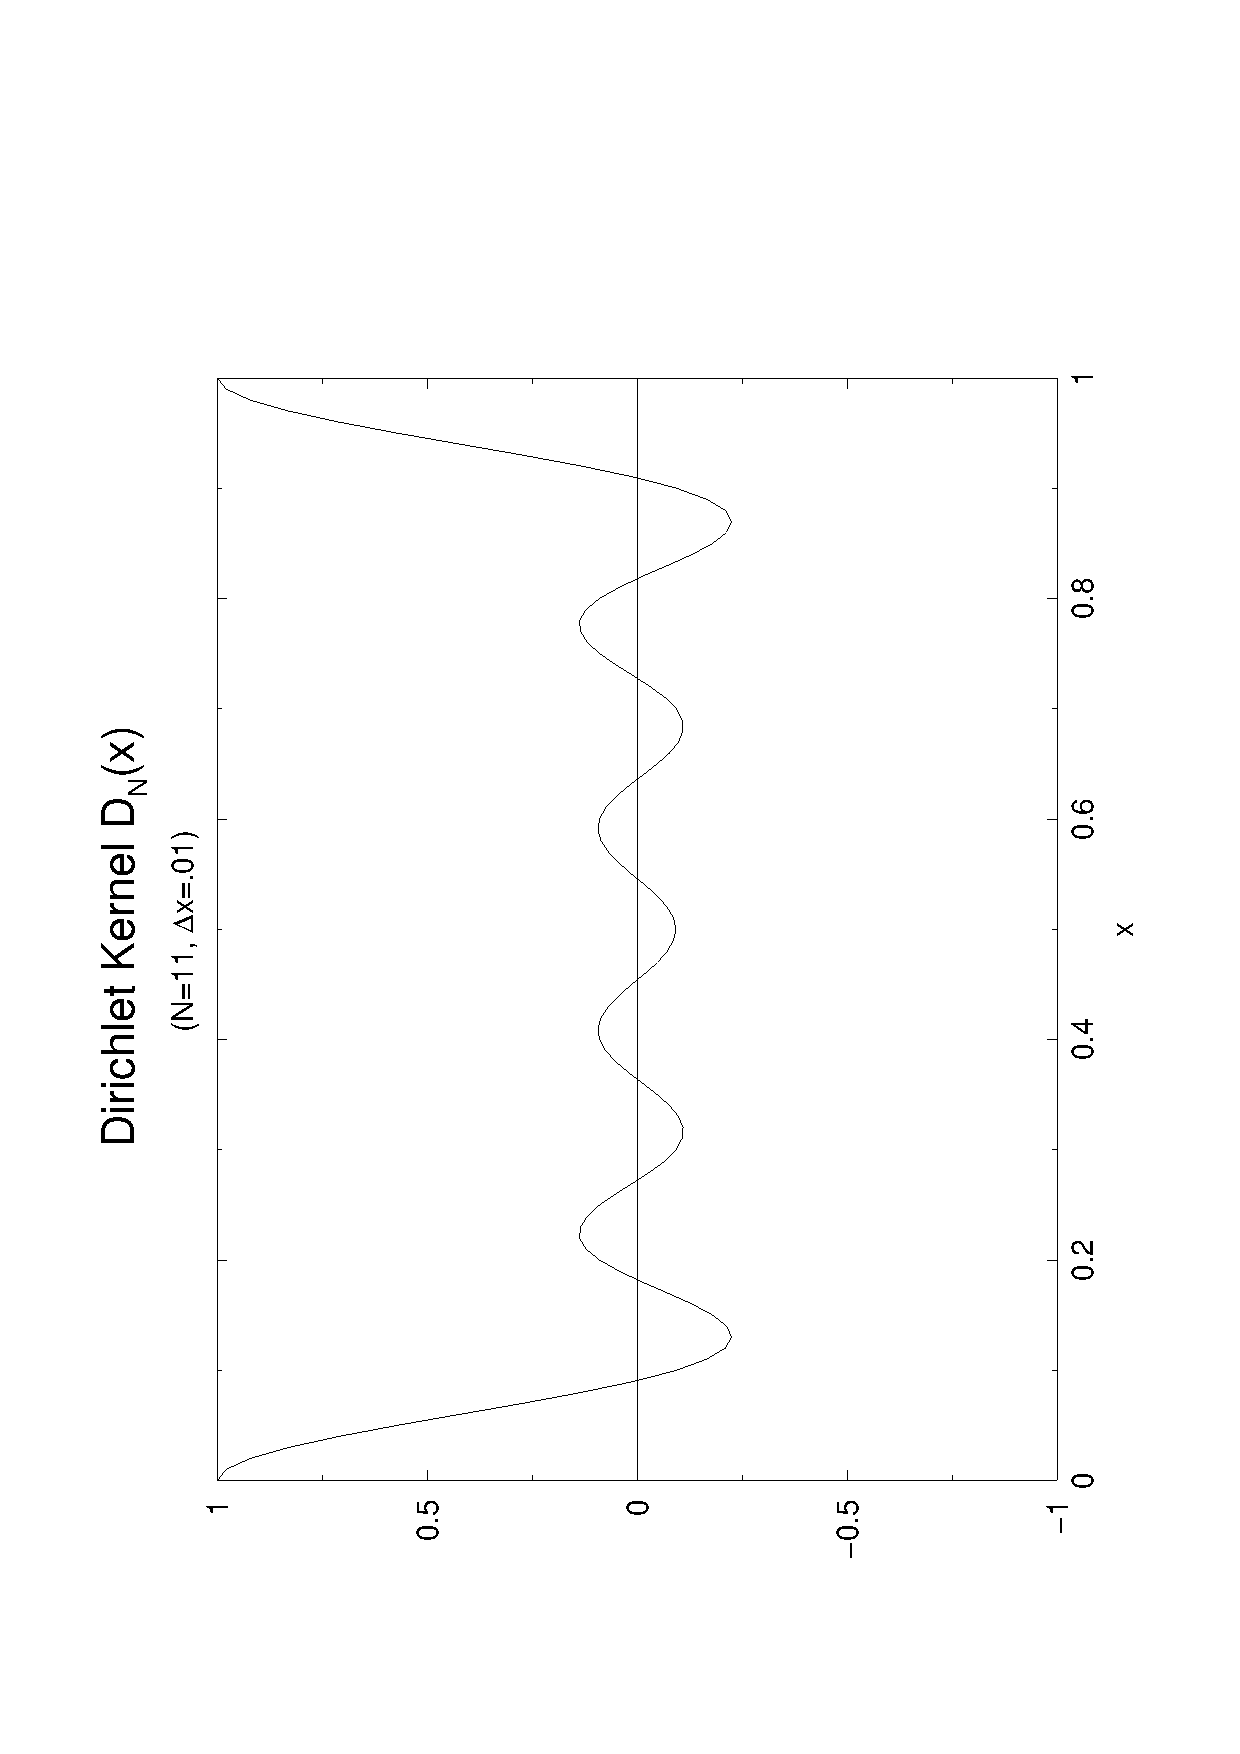
\includegraphics[angle=-90,width=4in]{fig2}
%{\psfig{file=fig3.ps,
%angle=-90,width=4in,bbllx=25pt,bblly=50pt,bburx=590pt,bbury=740pt}}
\caption{\label{f:fig3}
Dirichlet kernel for $N=10$, $\Delta x =.01$, and $0\le x\le 2$.}
\end{center}
\end{figure}
%

\end{document}
